\documentclass[tikz, border=10pt]{standalone}
\usepackage{tikz}
\usetikzlibrary{positioning, arrows.meta, backgrounds}

\tikzstyle{n} = [circle, draw, minimum size=0.8cm, align=center]

\begin{document}
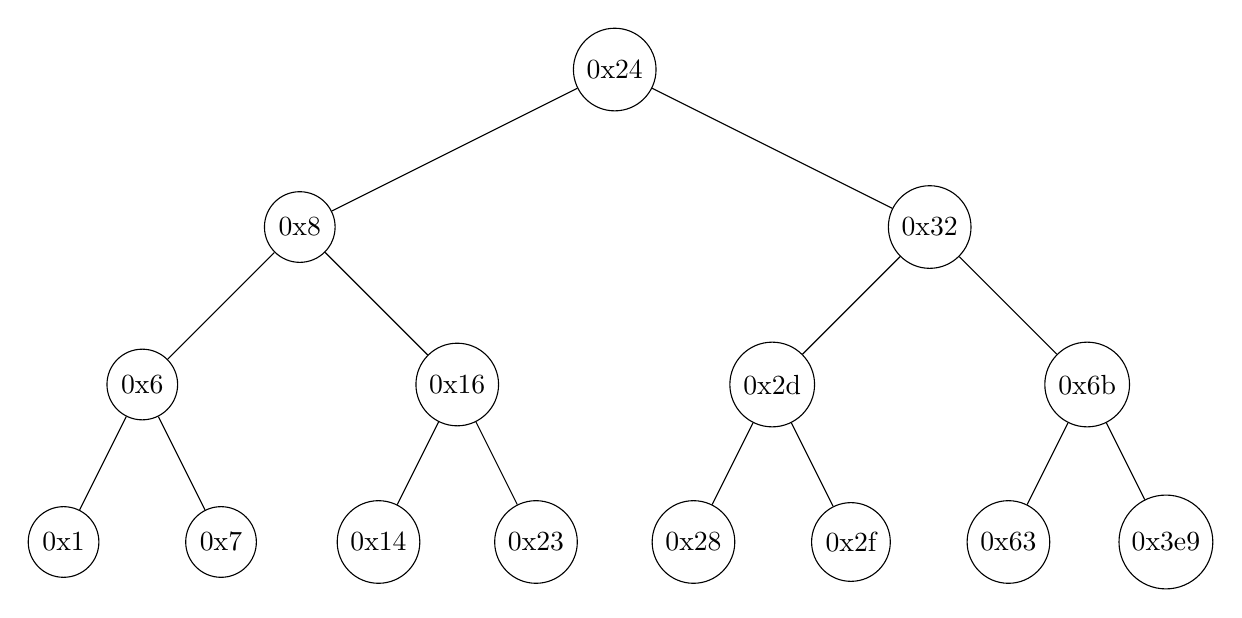
\begin{tikzpicture}[
    every node/.style={circle, draw, minimum size=0.8cm},
    level distance=20mm,
    level 1/.style={sibling distance=80mm},
    level 2/.style={sibling distance=40mm},
    level 3/.style={sibling distance=20mm}
]
    \node {0x24}
        child { node {0x8}
            child { node {0x6}
                child { node {0x1} }
                child { node {0x7} }
            }
            child { node {0x16}
                child { node {0x14} }
                child { node {0x23} }
            }
        }
        child { node {0x32}
            child { node {0x2d}
                child { node {0x28} }
                child { node {0x2f} }
            }
            child { node {0x6b}
                child { node {0x63} }
                child { node {0x3e9} }
            }
        };
\end{tikzpicture}
\end{document}